\section{Introduction}
A autonomous vehicle has as a main function to control all actors on its own.
This means that no human give a sign to the car that now its the time to turn the motor on.
To decide how the single components have to act at which time first the car need information about its own position which are as good as possible.
However, the next thing is to compute a path based on different informations.
For this problem there exist a big amount of solutions because for each type of vehicle there exist again a big amount of different algorithms to compute a path to another point.


\section{Position Calculation}


\subsection{Introduction}
One very important and critical part by the implementation of an autonomous vehicle is the calculation of the current position because there exist a big amount of problems which could not be solved.
This chapter contains on the one hand the different problems by creating a position calculating system and on the other one it describes methods to compute the best possible position.


\subsection{Position Specification}
One important part by calculating the current position is to specify how the current position have to be stored.
For this task there exist several types of structures.


\subsubsection{Cartesian Coordinate System}
The usual thing to storage a position is to storage the coordinates of the Cartesian coordinate system and also the angles how the object is aligned.
Also the 
This kind of storage has the advantage that is is very simple.
Also the memory and computing load efficiency is very good with this structure
The only disadvantage is that this structure doesn't contain the probability of the position and alternative positions.


\subsubsection{Probability Cloud}
This kind of the specification of a position have the disadvantage, that only the most possible position can be stored.
Another solution is to store a cloud of points with the different possibilities that this is the real position the the vehicle.

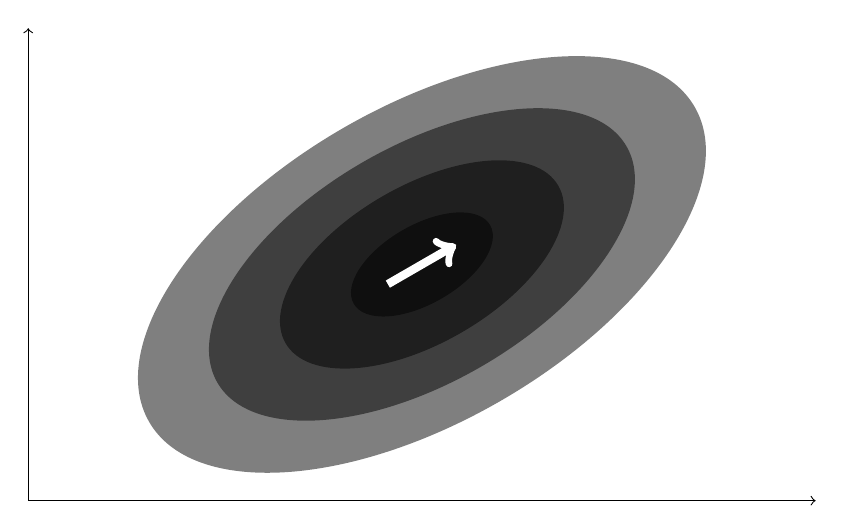
\begin{tikzpicture}
	\draw[->] (0,0) -- (10,0);
	\draw[->] (0,0) -- (0,6);
	\begin{scope}[shift={(5,3)},rotate=30]
		\foreach \x in {0,0.5,...,2}{
			\fill  [fill=black, semitransparent] (0,0) ellipse ({2 * \x} and {\x});
		}
		\draw[->,color=white,line width=3pt] (-0.5,0) -- +(1,0);
	\end{scope}
\end{tikzpicture}


\subsection{Sensors based Methods}


\subsubsection{Absolute Sensors}


\subsubsection{Relative Sensor}


\subsubsection{Environment Sensors}


\section{Path Calculation}


\subsection{Crawler Typed Vehicles}


\subsection{Car Like Vehicles}


\subsubsection{Path based on a circle}
\begin{figure}
\makebox[\linewidth]{
\begin{tikzpicture}[line cap=round,line join=round,>=triangle 45,x=1.0cm,y=1.0cm]
\draw[->,color=black] (-0.36,0) -- (9.32,0);
\foreach \x in {,2,4,6,8}
\draw[shift={(\x,0)},color=black] (0pt,2pt) -- (0pt,-2pt) node[below] {\footnotesize $\x$};
\draw[->,color=black] (0,-0.32) -- (0,4.18);
\foreach \y in {,2,4}
\draw[shift={(0,\y)},color=black] (2pt,0pt) -- (-2pt,0pt) node[left] {\footnotesize $\y$};
\draw[color=black] (0pt,-10pt) node[right] {\footnotesize $0$};
\clip(-0.36,-0.32) rectangle (9.32,4.18);
\draw (1,1)-- (9,1);
\draw[line width=1.6pt] (4.32,5.84) -- (6.32,5.84);
\draw [shift={(5,-4.17)}] plot[domain=0.91:2.23,variable=\t]({1*6.54*cos(\t r)+0*6.54*sin(\t r)},{0*6.54*cos(\t r)+1*6.54*sin(\t r)});
\draw [->] (1,1) -- (4.16,3.45);
\begin{scriptsize}
\fill [color=qqqqff] (1,1) circle (1.5pt);
\draw[color=qqqqff] (1.14,1.28) node {$A$};
\fill [color=qqqqff] (9,1) circle (1.5pt);
\draw[color=qqqqff] (9.16,1.28) node {$B$};
\fill [color=black] (5.53,5.84) circle (1.5pt);
\draw[color=black] (6.46,6.22) node {$Abfahrtswinkel = 0.66$};
\fill [color=uququq] (4.16,3.45) circle (1.5pt);
\draw[color=uququq] (4.72,3.72) node {$direction$};
\fill [color=uququq] (5,-4.17) circle (1.5pt);
\draw[color=uququq] (5.3,-3.9) node {$C_1$};
\end{scriptsize}
\end{tikzpicture}

\begin{tikzpicture}[line cap=round,line join=round,>=triangle 45,x=1.0cm,y=1.0cm]
\draw[->,color=black] (-0.36,0) -- (9.5,0);
\foreach \x in {,2,4,6,8}
\draw[shift={(\x,0)},color=black] (0pt,2pt) -- (0pt,-2pt) node[below] {\footnotesize $\x$};
\draw[->,color=black] (0,-0.38) -- (0,5.5);
\foreach \y in {,2,4}
\draw[shift={(0,\y)},color=black] (2pt,0pt) -- (-2pt,0pt) node[left] {\footnotesize $\y$};
\draw[color=black] (0pt,-10pt) node[right] {\footnotesize $0$};
\clip(-0.36,-0.38) rectangle (9.5,5.5);
\draw (1,1)-- (9,1);
\draw[line width=1.6pt] (4.32,5.84) -- (6.32,5.84);
\draw [shift={(5,1.35)}] plot[domain=-0.09:3.23,variable=\t]({1*4.02*cos(\t r)+0*4.02*sin(\t r)},{0*4.02*cos(\t r)+1*4.02*sin(\t r)});
\draw [->] (1,1) -- (0.65,4.98);
\begin{scriptsize}
\fill [color=qqqqff] (1,1) circle (1.5pt);
\draw[color=qqqqff] (1.14,1.28) node {$A$};
\fill [color=qqqqff] (9,1) circle (1.5pt);
\draw[color=qqqqff] (9.16,1.28) node {$B$};
\fill [color=black] (5.85,5.84) circle (1.5pt);
\draw[color=black] (6.78,6.22) node {$Abfahrtswinkel = 1.66$};
\fill [color=uququq] (0.65,4.98) circle (1.5pt);
\draw[color=uququq] (1.2,5.26) node {$direction$};
\fill [color=uququq] (5,1.35) circle (1.5pt);
\draw[color=uququq] (5.3,1.64) node {$C_1$};
\end{scriptsize}
\end{tikzpicture}
}
\caption{A to B path calculation}
\label{fig:AtoBcircle}
\end{figure}


\subsubsection{Path based on a circle and a line}
\begin{figure}
%A to B Circle Straight

\makebox[\linewidth]{
\begin{tikzpicture}[line cap=round,line join=round,>=triangle 45,x=1.0cm,y=1.0cm]
\draw[->,color=black] (-0.48,0) -- (10.48,0);
\foreach \x in {,2,4,6,8,10}
\draw[shift={(\x,0)},color=black] (0pt,2pt) -- (0pt,-2pt) node[below] {\footnotesize $\x$};
\draw[->,color=black] (0,-0.48) -- (0,6.24);
\foreach \y in {,2,4,6}
\draw[shift={(0,\y)},color=black] (2pt,0pt) -- (-2pt,0pt) node[left] {\footnotesize $\y$};
\draw[color=black] (0pt,-10pt) node[right] {\footnotesize $0$};
\clip(-0.48,-0.48) rectangle (10.48,6.24);
\draw [shift={(3,3)},color=qqwuqq,fill=qqwuqq,fill opacity=0.1] (0,0) -- (0:0.6) arc (0:225:0.6) -- cycle;
\draw[color=qqwuqq] (5.6,9.32) -- (7.04,9.32);
\draw [dash pattern=on 2pt off 2pt] (3,3)-- (10,3);
\draw(11.46,9.6) -- (13.46,9.6);
\draw [shift={(1.94,4.06)},color=qqwuqq]  plot[domain=1.25:5.5,variable=\t]({1*1.5*cos(\t r)+0*1.5*sin(\t r)},{0*1.5*cos(\t r)+1*1.5*sin(\t r)});
\draw [shift={(4.06,1.94)},color=qqqqcc]  plot[domain=2.36:5.14,variable=\t]({1*1.5*cos(\t r)+0*1.5*sin(\t r)},{0*1.5*cos(\t r)+1*1.5*sin(\t r)});
\draw [color=qqwuqq] (2.41,5.49)-- (10,3);
\draw [color=qqqqcc] (4.68,0.57)-- (10,3);
\begin{scriptsize}
\fill [color=qqqqff] (3,3) circle (1.5pt);
\draw[color=qqqqff] (3.14,3.28) node {$A$};
\fill [color=qqqqff] (10,3) circle (1.5pt);
\draw[color=qqqqff] (10.16,3.28) node {$B$};
\fill [color=qqwuqq] (6.5,9.32) circle (1.5pt);
\draw[color=qqwuqq] (7.46,9.7) node {$Abfahrtswinkel = 225\textrm{\degre}$};
\draw[color=qqwuqq] (3.06,3.4) node {$225\textrm{\degre}$};
\fill [color=black] (11.76,9.6) circle (1.5pt);
\draw[color=black] (12.78,9.98) node {$MinimalerRadius = 1.5$};
\end{scriptsize}
\end{tikzpicture}
}
\caption{A to B path calculation}
\label{fig:AtoBcircle}
\end{figure}


\subsubsection{Path based on a circle, a line and another circle}
\begin{figure}
%A to B Circle Straight Circle

\makebox[\linewidth]{
\begin{tikzpicture}[line cap=round,line join=round,>=triangle 45,x=1.0cm,y=1.0cm]
\draw[->,color=black] (-0.32,0) -- (12.44,0);
\foreach \x in {,2,4,6,8,10,12}
\draw[shift={(\x,0)},color=black] (0pt,2pt) -- (0pt,-2pt) node[below] {\footnotesize $\x$};
\draw[->,color=black] (0,-0.36) -- (0,6.14);
\foreach \y in {,2,4,6}
\draw[shift={(0,\y)},color=black] (2pt,0pt) -- (-2pt,0pt) node[left] {\footnotesize $\y$};
\draw[color=black] (0pt,-10pt) node[right] {\footnotesize $0$};
\clip(-0.32,-0.36) rectangle (12.44,6.14);
%\draw [shift={(3,3)},color=qqwuqq,fill=qqwuqq,fill opacity=0.1] (0,0) -- (0:0.6) arc (0:250:0.6) -- cycle;
%\draw [shift={(10,3)},color=qqwuqq,fill=qqwuqq,fill opacity=0.1] (0,0) -- (-35:0.6) arc (-35:180:0.6) -- cycle;
\draw[color=qqwuqq] (8.34,9.54) -- (9.78,9.54);
\draw[color=qqwuqq] (5.6,9.32) -- (7.04,9.32);
\draw [dash pattern=on 2pt off 2pt] (3,3)-- (10,3);
\draw(11.46,9.6) -- (13.46,9.6);
\draw [color=zzffqq] (1.47,5.01)-- (10.74,5.72);
\draw [shift={(1.59,3.51)},color=zzffqq]  plot[domain=1.65:5.93,variable=\t]({1*1.5*cos(\t r)+0*1.5*sin(\t r)},{0*1.5*cos(\t r)+1*1.5*sin(\t r)});
\draw [shift={(10.86,4.23)},color=zzffqq]  plot[domain=-2.18:1.65,variable=\t]({1*1.5*cos(\t r)+0*1.5*sin(\t r)},{0*1.5*cos(\t r)+1*1.5*sin(\t r)});
\draw [color=qqqqff] (4.19,1)-- (8.92,0.29);
\draw [color=ffdxqq] (8.26,0.55)-- (2.47,4.73);
\draw [color=ffqqqq] (9.86,5.35)-- (5.41,1.37);
\draw [shift={(4.41,2.49)},color=qqqqff]  plot[domain=2.79:4.56,variable=\t]({1*1.5*cos(\t r)+0*1.5*sin(\t r)},{0*1.5*cos(\t r)+1*1.5*sin(\t r)});
\draw [shift={(9.14,1.77)},color=qqqqff]  plot[domain=-1.72:0.96,variable=\t]({1*1.5*cos(\t r)+0*1.5*sin(\t r)},{0*1.5*cos(\t r)+1*1.5*sin(\t r)});
\draw [shift={(9.14,1.77)},color=ffdxqq]  plot[domain=-2.2:0.96,variable=\t]({1*1.5*cos(\t r)+0*1.5*sin(\t r)},{0*1.5*cos(\t r)+1*1.5*sin(\t r)});
\draw [shift={(1.59,3.51)},color=ffdxqq]  plot[domain=0.95:5.93,variable=\t]({1*1.5*cos(\t r)+0*1.5*sin(\t r)},{0*1.5*cos(\t r)+1*1.5*sin(\t r)});
\draw [shift={(4.41,2.49)},color=ffqqqq]  plot[domain=2.79:5.44,variable=\t]({1*1.5*cos(\t r)+0*1.5*sin(\t r)},{0*1.5*cos(\t r)+1*1.5*sin(\t r)});
\draw [shift={(10.86,4.23)},color=ffqqqq]  plot[domain=-2.18:2.3,variable=\t]({1*1.5*cos(\t r)+0*1.5*sin(\t r)},{0*1.5*cos(\t r)+1*1.5*sin(\t r)});
\begin{scriptsize}
\fill [color=qqqqff] (3,3) circle (1.5pt);
\draw[color=qqqqff] (3.14,3.28) node {$A$};
\fill [color=qqqqff] (10,3) circle (1.5pt);
\draw[color=qqqqff] (10.16,3.28) node {$B$};
\fill [color=qqwuqq] (9.2,9.54) circle (1.5pt);
%\draw[color=qqwuqq] (10.18,9.92) node {$Ankunftswinkel = 215\textrm{\degre}$};
\fill [color=qqwuqq] (6.6,9.32) circle (1.5pt);
%\draw[color=qqwuqq] (7.56,9.7) node {$Abfahrtswinkel = 250\textrm{\degre}$};
%\draw[color=qqwuqq] (2.98,3.36) node {$250\textrm{\degre}$};
%\draw[color=qqwuqq] (10.3,3.4) node {$215\textrm{\degre}$};
\fill [color=black] (11.76,9.6) circle (1.5pt);
\draw[color=black] (12.78,9.98) node {$MinimalerRadius = 1.5$};
\end{scriptsize}
\end{tikzpicture}
}

\caption{A to B path calculation}
\label{fig:AtoBcircle}
\end{figure}